\documentclass[tikz, crop, border = {2pt 2pt 2pt 2pt}]{standalone}

\usetikzlibrary{decorations.pathreplacing, decorations.text, calc}
\usepackage{physics}
\usepackage{concmath-otf}

\begin{document}
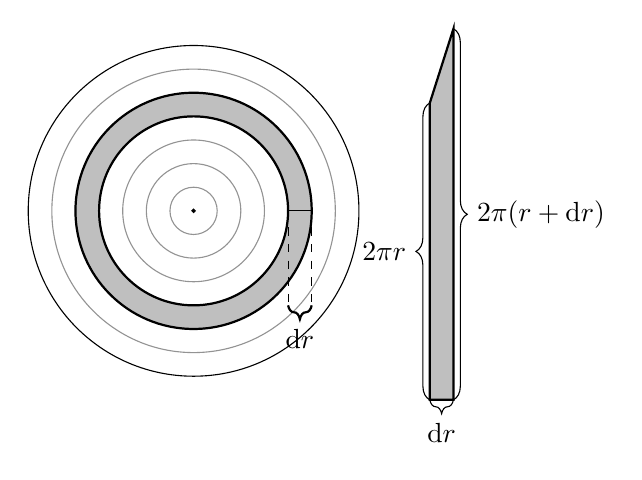
\begin{tikzpicture}[scale = 0.6]
    \draw (0, 0) circle (3.5);
    \filldraw (0, 0) circle (1pt);
    \foreach \x in {0.5, 1, ..., 3} {
        \draw[gray!85] (0, 0) circle (\x);
    }

    \filldraw[even odd rule, fill = lightgray, draw = black, blend mode = multiply, thick] (0, 0) circle (2) (0, 0) circle (2.5);
    \draw[dashed] (2, 0) -- ++ (0, -2) (2.5, 0) -- ++ (0, -2);
    \draw[decorate, decoration = {brace, amplitude = 5pt, mirror}, thick] (2, -2) -- ++ (0.5, 0) node[below = 5pt, midway]{$\dd{r}$};
    \draw (2, 0) -- ++ (0.5, 0);

    \begin{scope}[shift = ({5, -4})]
        \filldraw[draw = black, fill = lightgray, thick] (0, 0) -- ++ (0, {2*pi}) -- (0.5, {2.5*pi}) -- (0.5, 0) -- cycle;
        \draw[decorate, decoration = {brace, amplitude = 5pt, mirror}] (0, 0) -- (0.5, 0) node[below = 5pt, midway]{$\dd{r}$};
        \draw[decorate, decoration = {brace, amplitude = 5pt}] (0, 0) -- ++ (0, {2*pi}) node[left = 5pt, midway]{$2\pi r$};
        \draw[decorate, decoration = {brace, amplitude = 5pt, mirror}] (0.5, 0) -- ++ (0, {2.5*pi}) node[right = 5pt, midway]{$2\pi(r + \dd{r})$};
    \end{scope}
\end{tikzpicture}
\end{document}